\documentclass[bachelor, och, labwork]{shiza}
% параметр - тип обучения - одно из значений:
%    spec     - специальность
%    bachelor - бакалавриат (по умолчанию)
%    master   - магистратура
% параметр - форма обучения - одно из значений:
%    och   - очное (по умолчанию)
%    zaoch - заочное
% параметр - тип работы - одно из значений:
%    referat    - реферат
%    coursework - курсовая работа (по умолчанию)
%    diploma    - дипломная работа
%    pract      - отчет по практике
% параметр - включение шрифта
%    times    - включение шрифта Times New Roman (если установлен)
%               по умолчанию выключен
\usepackage{subfigure}
\usepackage{tikz,pgfplots}
\pgfplotsset{compat=1.5}
\usepackage{float}

%\usepackage{titlesec}
\setcounter{secnumdepth}{4}
%\titleformat{\paragraph}
%{\normalfont\normalsize}{\theparagraph}{1em}{}
%\titlespacing*{\paragraph}
%{35.5pt}{3.25ex plus 1ex minus .2ex}{1.5ex plus .2ex}

\titleformat{\paragraph}[block]
{\hspace{1.25cm}\normalfont}
{\theparagraph}{1ex}{}
\titlespacing{\paragraph}
{0cm}{2ex plus 1ex minus .2ex}{.4ex plus.2ex}

% --------------------------------------------------------------------------%


\usepackage[T2A]{fontenc}
\usepackage[utf8]{inputenc}
\usepackage{graphicx}
\graphicspath{ {./images/} }
\usepackage{tempora}

\usepackage[sort,compress]{cite}
\usepackage{amsmath}
\usepackage{amssymb}
\usepackage{amsthm}
\usepackage{fancyvrb}
\usepackage{listings}
\usepackage{listingsutf8}
\usepackage{longtable}
\usepackage{array}
\usepackage[english,russian]{babel}

% \usepackage[colorlinks=true]{hyperref}
\usepackage{url}

\usepackage{underscore}
\usepackage{setspace}
\usepackage{indentfirst} 
\usepackage{mathtools}
\usepackage{amsfonts}
\usepackage{enumitem}
\usepackage{tikz}

\newcommand{\eqdef}{\stackrel {\rm def}{=}}
\newcommand{\specialcell}[2][c]{%
\begin{tabular}[#1]{@{}c@{}}#2\end{tabular}}

\renewcommand\theFancyVerbLine{\small\arabic{FancyVerbLine}}

\newtheorem{lem}{Лемма}

\begin{document}

% Кафедра (в родительном падеже)
\chair{}

% Тема работы
\title{Сетевая утилита arp}

% Курс
\course{2}

% Группа
\group{231}

% Факультет (в родительном падеже) (по умолчанию "факультета КНиИТ")
\department{факультета КНиИТ}

% Специальность/направление код - наименование
%\napravlenie{09.03.04 "--- Программная инженерия}
%\napravlenie{010500 "--- Математическое обеспечение и администрирование информационных систем}
%\napravlenie{230100 "--- Информатика и вычислительная техника}
%\napravlenie{231000 "--- Программная инженерия}
\napravlenie{100501 "--- Компьютерная безопасность}

% Для студентки. Для работы студента следующая команда не нужна.
% \studenttitle{Студентки}

% Фамилия, имя, отчество в родительном падеже
\author{Окунькова Сергея Викторовича}

% Заведующий кафедрой
% \chtitle{} % степень, звание
% \chname{}

%Научный руководитель (для реферата преподаватель проверяющий работу)
\satitle{ассистент} %должность, степень, звание
\saname{А. А. Фомин}

% Руководитель практики от организации (только для практики,
% для остальных типов работ не используется)
% \patitle{к.ф.-м.н.}
% \paname{С.~В.~Миронов}

% Семестр (только для практики, для остальных
% типов работ не используется)
%\term{8}

% Наименование практики (только для практики, для остальных
% типов работ не используется)
%\practtype{преддипломная}

% Продолжительность практики (количество недель) (только для практики,
% для остальных типов работ не используется)
%\duration{4}

% Даты начала и окончания практики (только для практики, для остальных
% типов работ не используется)
%\practStart{30.04.2019}
%\practFinish{27.05.2019}

% Год выполнения отчета
\date{2021}

\maketitle

% Включение нумерации рисунков, формул и таблиц по разделам
% (по умолчанию - нумерация сквозная)
% (допускается оба вида нумерации)
% \secNumbering

%-------------------------------------------------------------------------------------------


\begin{enumerate}
    
    \item Воспользовавшись командой arp просмотрите arp таблицу вашего компьютера.
    
    \begin{figure}[H]
        \centering      %размер рисунка       здесь находится название файла рисунка, без указания формата
        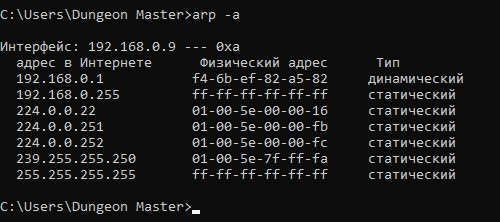
\includegraphics[width=0.75\textwidth]{1}
        \caption{Таблица arp моего компьютера}
        \label{fig:image1}
    \end{figure}

    \item Определите MAC адрес шлюза вашей локальной сети.
    
    Моим MAC адресом шлюза локальной сети является адрес f4-6b-ef-82-a5-82

    \item Определите MAC адрес любого из компьютеров вашего класса.
    
    \begin{figure}[H]
        \centering      %размер рисунка       здесь находится название файла рисунка, без указания формата
        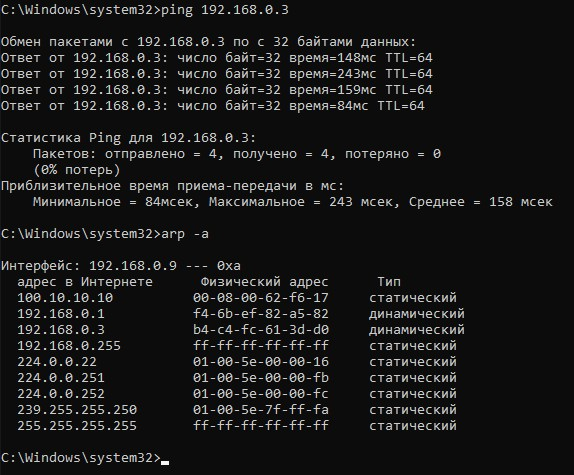
\includegraphics[width=0.75\textwidth]{2}
        \caption{Поиск компьютера моего класса}
        \label{fig:image1}
    \end{figure}
    
    MAC адрес компьютера из моего класса : b4-c4-fc-61-3d-d0

    \item Внесите в arp таблицу заведомо неправильное значение для MAC адреса этого компьютера. Проверьте его 
    доступность с помощью утилиты ping. Прокомментируйте результат.

    \begin{figure}[H]
        \centering      %размер рисунка       здесь находится название файла рисунка, без указания формата
        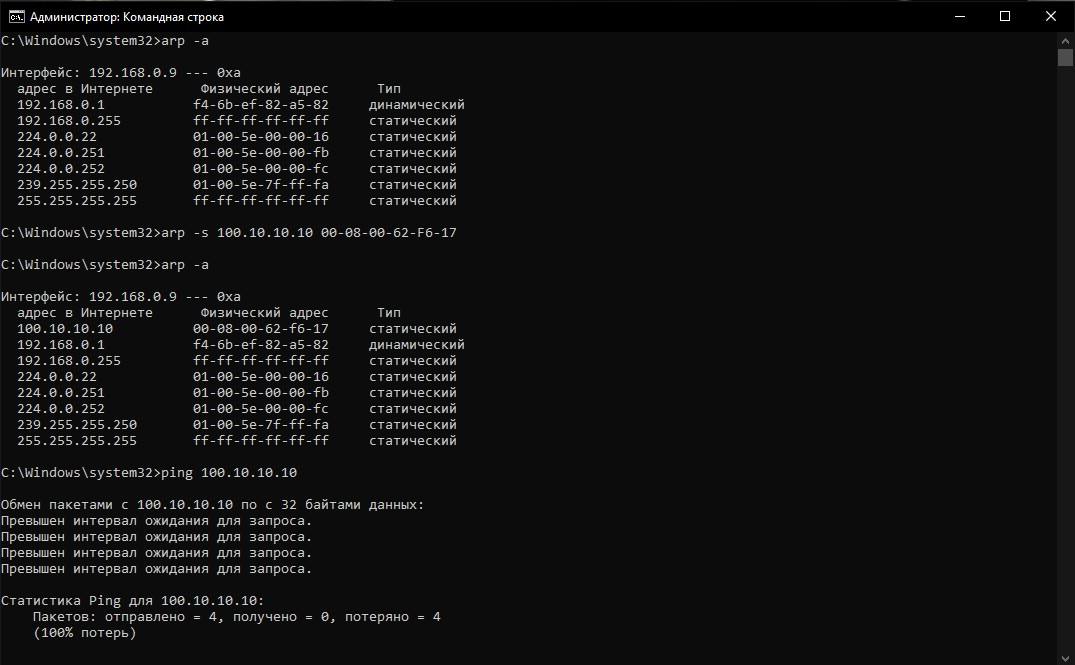
\includegraphics[width=0.75\textwidth]{3}
        \caption{Внесение в arp таблицу неправильное значение для MAC адреса этого компьютера и проверка его доступности}
        \label{fig:image1}
    \end{figure}

    Неправильное значение для MAC адреса этого компьютера появилось, но оно не доступно, поэтому мы только теряем пакеты.

    \item Очистите arp таблицу. Выполните утилиту ping на тот же компьютер. Выведите таблицу arp и прокомментируйте результат.
    
    \begin{figure}[H]
        \centering      %размер рисунка       здесь находится название файла рисунка, без указания формата
        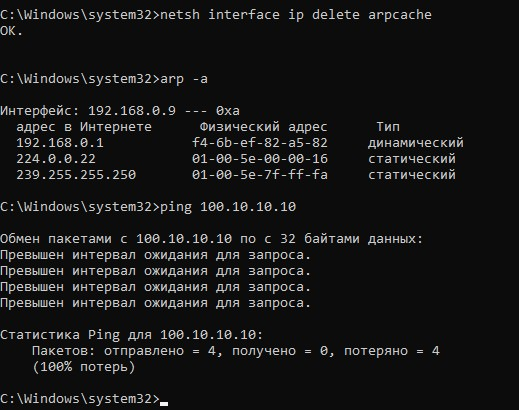
\includegraphics[width=0.75\textwidth]{4}
        \caption{Очистка arp таблицы}
        \label{fig:image1}
    \end{figure}

\end{enumerate}

\end{document}
